\documentclass[12pt]{article}
\usepackage{amsmath}
\usepackage{amssymb,float}
\usepackage{graphicx}
\usepackage{subcaption}
\usepackage{hyperref}
\usepackage{flexisym}
\usepackage{color}
\usepackage{breqn}
\usepackage{rotating}
\usepackage{tikz}
\usepackage[utf8]{inputenc}
\usepackage{tabularx, blkarray}
\usepackage[linesnumbered,boxed]{algorithm2e}
\newcommand\colhead[1]{\multicolumn{1}{>{$}c<{$}}{#1}}
\usepackage{eqparbox}
\usepackage{listings}
\definecolor{mygreen}{RGB}{28,172,0} % color values Red, Green, Blue
\definecolor{mylilas}{RGB}{170,55,241}
\lstset{language=Matlab,%
    %basicstyle=\color{red},
    breaklines=true,%
    morekeywords={matlab2tikz},
    keywordstyle=\color{blue},%
    morekeywords=[2]{1}, keywordstyle=[2]{\color{black}},
    identifierstyle=\color{black},%
    stringstyle=\color{mylilas},
    commentstyle=\color{mygreen},%
    showstringspaces=false,%without this there will be a symbol in the places where there is a space
    numbers=left,%
    numberstyle={\tiny \color{black}},% size of the numbers
    numbersep=9pt, % this defines how far the numbers are from the text
    emph=[1]{for,end,break},emphstyle=[1]\color{red}, %some words to emphasise
    %emph=[2]{word1,word2}, emphstyle=[2]{style},    
}
\newcommand*{\captionsource}[2]{%
  \caption[{#1}]{%
    #1%
    \\\hspace{\linewidth}%
    \textbf{Source:} #2%
  }%
}

\newcommand{\Rea}{{\Bbb R}}
\newcommand{\Int}{{\Bbb Z}}
\newcommand{\Rat}{{\Bbb Q}}
\newcommand{\Cmp}{{\Bbb C}}
\newcommand{\Nat}{{\Bbb N}}

\setlength{\oddsidemargin}{.25in} \setlength{\evensidemargin}{.25in}
\setlength{\textwidth}{6in} \setlength{\topmargin}{0.0in}
\setlength{\textheight}{8.5in}

\newtheorem{definition}{Definition}
\newtheorem{remark}{Remark}
\newtheorem{theorem}{Theorem}
\newtheorem{lemma}[theorem]{Lemma}
\newtheorem{corollary}[theorem]{Corollary}
\newtheorem{proposition}[theorem]{Proposition}
\newtheorem{claim}[theorem]{Claim}
\newtheorem{observation}{Observation}
\newtheorem{fact}{Fact}

\newenvironment{proof}{\noindent{\bf Proof:} \hspace*{1em}}{
    \hspace*{\fill} $\Box$ }
\newenvironment{proof_of}[1]{\noindent {\bf Proof of #1:}
    \hspace*{1em} }{\hspace*{\fill} $\Box$ }
\newenvironment{proof_claim}{\begin{quotation} \noindent}{
    \hspace*{\fill} $\diamond$ \end{quotation}}


\newcommand{\handout}[5]{
   \renewcommand{\thepage}{#1-\arabic{page}}
   \noindent
   \begin{center}
   \framebox{
      \vbox{
    \hbox to 5.78in { {\bf ORIE 4741 Learning with Big Messy Data} \hfill #2 }
       \vspace{4mm}
       \hbox to 5.78in { {\Large \hfill #5  \hfill} }
       \vspace{2mm}
       \hbox to 5.78in { {\it #3 \hfill #4} }
      }
   }
   \end{center}
   \vspace*{4mm}
}

\newcommand{\Assignment}[4]{\handout{#1}{#2}{Assignment:
#3}{Student: #4}{Assignment #1}}
\newcommand{\problemset}[4]{\handout{#1}{#2}{}{Due Date: #4}{Problem Set #3}}
\newcommand{\problemsetsoln}[3]{\handout{#1}{#2}{}{}{Problem Set #3 Solutions}}
\newcommand{\exam}[3]{\handout{#1}{#2}{}{Due Date: #3}{Take-Home Final Exam}}
\newcommand{\examsoln}[2]{\handout{#1}{#2}{}{}{Take-Home Final Exam Solutions}}

\newcommand{\OPT}{\operatorname{OPT}}
\newcommand{\set}[1]{\{#1\}}


\newcommand{\dpw}{}

\newenvironment{alglist}{\begin{list}{}{\setlength{\leftmargin}{1.5cm}
\setlength{\rightmargin}{0cm}\setlength{\itemsep}{1ex}\setlength{\parsep}{1ex}}}{\end{list}}

\newcommand{\problem}[3]
{\fbox{\parbox{6in}{{\bf #1}\begin{itemize}\item{\bf Input:} {#2} \item{\bf Goal:} {#3}\end{itemize}}}}



\begin{document}

%%%%%%%%%%%%%%%%%%%%%
%	                 TITLE BOX
%%%%%%%%%%%%%%%%%%%%%

\Assignment{1}{Sep. 12, 2017}{\dpw}{Faisal Alkaabneh}

%%%%%%%%%%%%%%%%%%%%%
%	             First Section
%%%%%%%%%%%%%%%%%%%%%


\section{Problem 1}
\textcolor{red}{\textit{Vectors, matrices and inner products}.}\\

\begin{itemize}
\item After running this: $u = rand(3,1);v = rand(3,1); u'v$ the result is as follows 1*1Array $\lbrace$Float64,2$\rbrace$:
 $0.993625$. On the other hand, running the following $x = rand(3); y = rand(3); x'*y$ provided the following result: $0.91015084477077$. The size of the former result is $(1,1)$ whereas the size of the later result is Epmty! Cearly, Julia distingushes between elements multiplications vs array multiplications. 
\item In the case of using dot vs sum functions for vectors $u$ and $v$, the results are exactly the same, we got a scalar. Likewise, for the case of vectors $x$ and $y$. 
\item The results I got after running A[1,:] vs A[:,1] was, surprisingly, the same. The result is always a 5-element Array. Frankly speaking, I was expecting to get a column vector and a row vectors respectively just like what you get in MATLAB! Clearly, the answer is we get vectors.
\item sum(A[:,1].*A[1,:]) or dot(A[:,1],A[1,:]).
\end{itemize}



\newpage


\section{Problem 3}
\textcolor{red}{Perceptron.}

\vspace{0.2 in}
\begin{itemize}
    \item[(a)] The code is displayed in Figure \ref{fig:perCode}.
    \item[(b)] The number of steps required was 48 iterations before converging. For the plots please see Figure \ref{fig:vs}
    \item[(c)] I noticed first that there is a significant difference between the number of steps needed to converge for the same set of data since the initial $w$ is random. Nonetheless, here are the reutls for $n= 20,100,$ and $1000$: 4, 64, and 115. Clearly as n goes up, the number of steps required for convergence goes up as well.
    \item[(d)] 96, 500, 392, 475, 500, 500, 387, 334.
    \item[(e)] Figure displays the number of iterations needed by the algorithm at different data points. Also Figure XX shows the code used. Note that the maximum value is 439 and the minimum is 68.
    \item[(f)]
    \item[()]
\end{itemize}


\begin{figure}[H]
\centering
    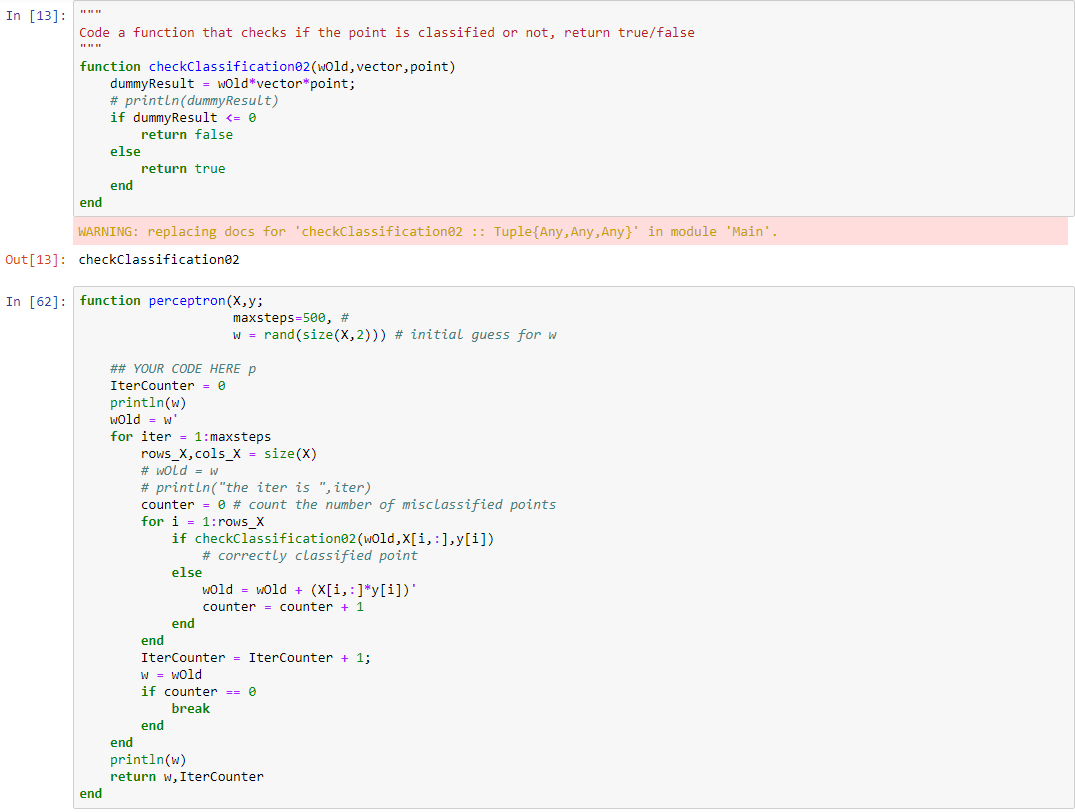
\includegraphics[width=450 pt]{perAlgo.png}
    \caption{Problem 3 part (a).}
    \label{fig:perCode}
\end{figure}


\begin{figure}[H]
\centering
    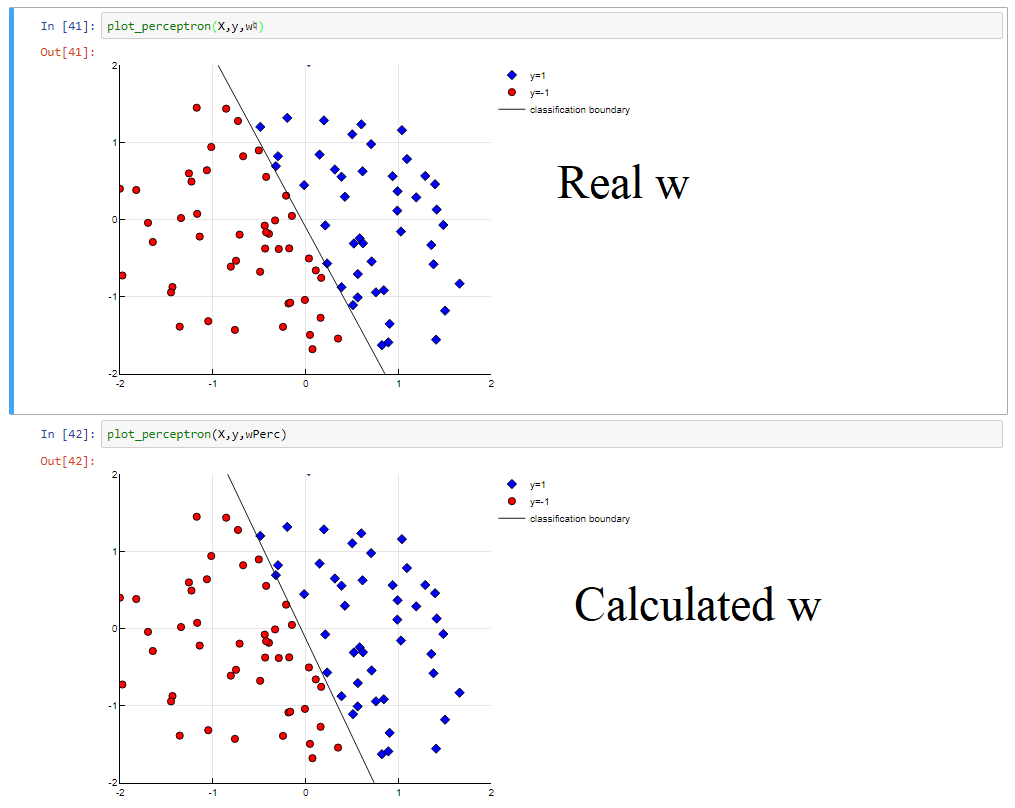
\includegraphics[width=450 pt]{realvshypo.png}
    \caption{Problem 3: $w\natural$ vs $w$ predicted.}
    \label{fig:vs}
\end{figure}


\begin{figure}[H]
\centering
    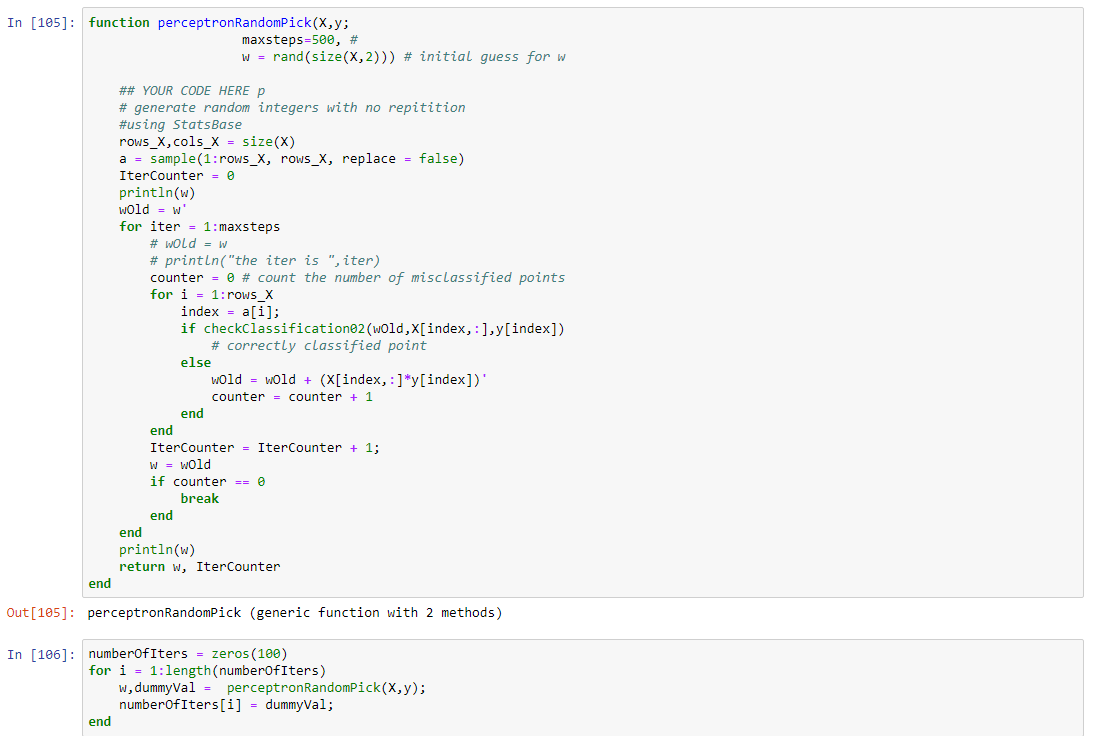
\includegraphics[width=450 pt]{perAlgoRand.png}
    \caption{Problem 3: Perceptron algorithm with random pick of the next point to evaluate.}
    \label{fig:vs}
\end{figure}


\begin{figure}[H]
\centering
    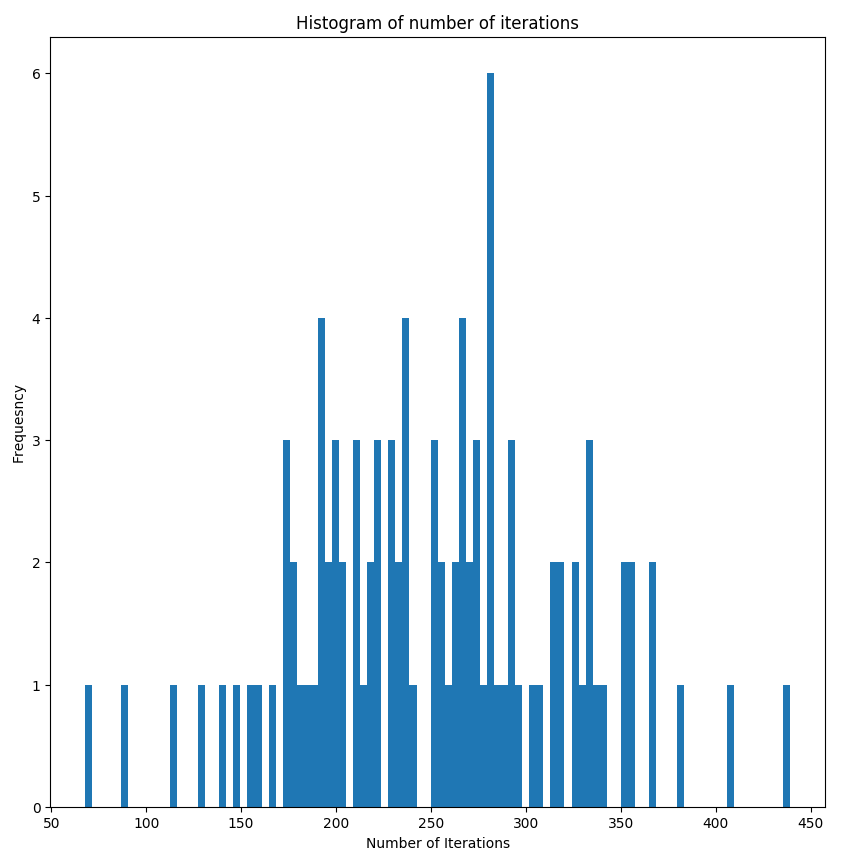
\includegraphics[width=450 pt]{freq.png}
    \caption{Problem 3: frequescy..........}
    \label{fig:vs}
\end{figure}


\end{document}
